\author{João Gonçalves}
\newcommand{\authorD}{Daniel Dinis}
\newcommand{\authorM}{Martim Bento}
\newcommand{\authorT}{Tiago Brogueira}
\newcommand{\studentID}{99995}
\newcommand{\studentIDD}{99906}
\newcommand{\studentIDM}{100031}
\newcommand{\studentIDT}{100095}
\newcommand{\supervisorone}{Prof\textsuperscript{\underline{a}}. Célia Jesus}
\newcommand{\supervisortwo}{}
\newcommand{\department}{Engenharia Eletrotécnica e de Computadores}
\newcommand{\exam}{Electrotecnia Teórica}

\title{%
4\textsuperscript{\underline{o}} Trabalho Laboratorial\\
\large REGIMES TRANSITÓRIOS}
\date{Abril 2022}

\documentclass[a4paper,12pt]{article}
\usepackage[left=30mm,top=30mm,right=30mm,bottom=30mm]{geometry}
\usepackage{etoolbox}
\usepackage{pgfplots}
\usepackage{circuitikz}
\usepackage{booktabs}
\usepackage[usestackEOL]{stackengine}
\usepackage[T1]{fontenc}
\usepackage[utf8]{inputenc}
\usepackage{bm}
\usepackage[export]{adjustbox}
\usepackage{graphicx}
\usepackage{subcaption}
\usepackage{amsmath}
\usepackage{amsfonts}
\usepackage{mathtools}
%\usepackage[svgnames]{xcolor}
\usepackage{float}
\usepackage{hyperref}
\usepackage[capitalise]{cleveref}
\usepackage{enumitem,kantlipsum}
\usepackage[square,numbers,sort]{natbib}
\usepackage[ruled,vlined]{algorithm2e}
\usepackage{listings}
\usepackage{minted}
\usepackage{amssymb}
\usepackage{babel}
\usepackage[bottom]{footmisc}
\usemintedstyle{emacs}
%\setlength{\parindent}{0pt}

\renewcommand{\listingscaption}{Algorithm}
\renewcommand{\listoflistingscaption}{List of Algorithms}
\renewcommand{\figurename}{Fig.}
\renewcommand{\tablename}{Tab.}
\renewcommand{\contentsname}{Índice}

\bibliographystyle{unsrtnat}

\hypersetup{
    colorlinks,
    linkcolor={black},
    citecolor={blue!50!black},
    urlcolor={blue!80!black}
}

\linespread{1}

\newtheorem{theorem}{Theorem}[section]
\graphicspath{{figures/}}	

%----------------------------------TITLE PAGE -----------------------------------
\makeatletter
\def\maketitle{
  \begin{center}\leavevmode
       \normalfont
       
\includegraphics[width=0.55\columnwidth]{IST.pdf}
       \vskip 1.5cm   
       \textsc{\large \department}\\
       \vskip 1.5cm
       \rule{\linewidth}{0.2 mm} %\\
       {\large \exam}\\[1 cm]
       {\huge \bfseries \@title \par}
       \vspace{1cm}
	\rule{\linewidth}{0.2 mm} \\[1.5 cm]
	 
	\begin{minipage}[t]{0.45\textwidth}
		\begin{flushleft} \large
			\emph{Autores:}\\
            \textbf{\authorD} : \studentIDD\\
			\textbf{\@author} : \studentID\\
            \textbf{\authorM} : \studentIDM\\
			\textbf{\authorT} : \studentIDT
		\end{flushleft}
	\end{minipage}
	\begin{minipage}[t]{0.45\textwidth}
	   \begin{flushright} \large
			\ifdefempty{\supervisortwo}{\emph{Supervisora:\\}}{\emph{Supervisores:\\}}
			\supervisorone\\
			\ifdefempty{\supervisortwo}{}{\supervisortwo\\}
		\end{flushright}
	\end{minipage}
	\vfill
	{\Large \@date\par}
   \end{center}
   %\vfill
   %\null
   \cleardoublepage
  }
\makeatother
%-------------------------------- ENDTITLE PAGE ----------------------------------

\pgfplotsset{compat=1.18}
\begin{document}

    %% title page
    \pagenumbering{gobble}
    \maketitle
    %% body
    \newpage
    \pagenumbering{arabic}
    \section*{Questões}
    %\clearpage
\def\delequal{\mathrel{\ensurestackMath{\stackon[1pt]{=}{\scriptstyle\Delta}}}}
%//==============================--@--==============================//%
\subsection*{\underline{2.1} Circuito RL Série}
%//==============================--A--==============================//%
\subsubsection*{(a) Obtenha o regime transitório relativo à corrente $i$ para $t \ge 0$.}
\label{subsubsec_a}
\paragraph{Resposta:}
Por aplicação direta da Lei de Indução, $\overrightarrow{\nabla} \times \overrightarrow{E} = -\dfrac{\partial}{\partial t}\overrightarrow{B}$, é facilmente derivada a EDO linear de primeiro grau que rege o sistema. Naturalmente, como o gerador não impõe nenhuma tensão para $t < 0$, verifica-se o seguinte par:

$$
    \begin{cases}
        u_g(t) = i(t)R + L \dfrac{di(t)}{dt} \\
        i(0^-) = i(0^+) = 0
    \end{cases}
$$

Deste modo, procura-se a solução homogénea (\textit{natural}), $i_n(t)$, e a solução particular (\textit{forçada}), $i_f(t)$, tal que a resposta do PVI se verifique pela justaposição das soluções mencionadas, i.e.:

\begin{equation}
    \label{eq1}
    i(t) = i_n(t) + i_f(t)
\end{equation}

\noindent
\underline{Solução natural:} 

A equação linear homogénea $L \dfrac{di(t)}{dt} + i(t)R = 0$, tem como equação característica: 

$$
    Ls + R = 0 \iff s = -\frac{R}{L} \implies \tau = -\frac{1}{s} = \frac{L}{R} = \frac{1}{3000} = 0.(3)\ \text{ms} 
$$
$$
    \therefore i_n(t) = I_n e^{-t/\tau}\ \text{A}
$$

\vspace{0.5cm}
\noindent
\underline{Solução forçada:}
\vspace{0.25cm}

No domínio dos fasores é trivialmente deduzida a resposta forçada. Atendendo à equação que rege o circuito no domínio do tempo, observa-se:

$$
    \bar{U}_g = R \bar{I}_f + j\omega L \bar{I}_f = \bar{Z}_{eq} \bar{I}_f \implies \bar{I}_f = \frac{\bar{U}_g}{\bar{Z}_{eq}} = \frac{U_g}{Z_{eq}}e^{j(\alpha - \measuredangle \bar{Z}_{eq})}
$$

$$
\implies i_f(t) = \frac{U_g}{Z_{eq}} \cos{(\omega t + \alpha - \measuredangle \bar{Z}_{eq})} = I_f \cos{(\omega t + \alpha - \varphi)}
$$

$$
    \begin{cases}
        I_f = U_g/\sqrt{R^2+(\omega L)^2} \approx 0.634 \sqrt{2}\ \text{mA} \\
        \varphi = \measuredangle \bar{Z}_{eq} = \arctan{(\dfrac{\omega L}{R})} \approx 1.476\ \text{rad}
    \end{cases}
$$

$$
    \therefore i_f(t) \approx 0.634 \sqrt{2}\cdot \cos{(\omega t - 3.046)}\ \text{mA}\text{, para $\alpha = -\pi/2$.}
$$

\clearpage
Com especial atenção ao enunciado em \hyperref[eq1]{(1)} e às condições iniciais do PVI, procede-se à determinação do valor inicial do regime \textit{natural} para que se obtenha a solução geral da equação diferencial (i.e., $i(t)$).

$$
    i(0) = 0 \iff i_n(0) = -i_f(0) \implies I_n = -0.634\sqrt{2}\cdot \cos{(-3.046)} \cdot 10^{-3}
$$

$$
    \implies I_n \approx 0.893\ \text{mA}
$$

$$
    \therefore i(t) = 0.634\sqrt{2}\cdot [\ \cos{(\omega t - 3.046)} - \cos{(3.046)}\cdot e^{-3000t}\ ]\ \text{mA}
$$
\hfill \ensuremath{\Box}
%//==============================--B--==============================//%
\subsubsection*{(b) Determine a expressão que permite calcular aproximadamente os instantes em que a corrente $i$ tem extremos, supondo que estes extremos se dão quando $\cos{(\omega t + \alpha - \varphi)} = \pm 1$, e
determine também a expressão que permite determinar o valor desses extremos para
$\alpha = -\pi/2$.}
\label{subsubsec_b}
\paragraph{Resposta:}
Tomando a aproximação enunciada, encontramos os extremos quando a expressão $\cos{(\omega t_x + \alpha - \varphi)} = \pm 1$ se verifica. Deste modo, é uma reação imediata\footnotemark concluir que:

$$
    \omega t_x + \alpha -\varphi = k\pi\text{,}\ \forall k \in \mathbb{Z}_{0}^{+}
$$

Assim, os instantes $t_x$ correspondentes aos e\textbf{x}tremos (para $\alpha = -\pi/2$) são:

$$
    \implies t_x = \frac{k\pi - \alpha + \varphi}{\omega} \iff t_x = \frac{k\pi + 3.046}{10000\pi} \approx (100k + 96.957)\ \mu\text{s}\text{,}\ \forall k \in \mathbb{Z} 
$$

Segue-se que a expressão que nos permite calcular os extremos (\textit{aproximadamente}) pode ser descrita por:

$$
    i(t_x) = 0.634\sqrt{2}\cdot [\ (-1)^k - \cos{(3.046)}\cdot e^{-3(100k + 96.957)\cdot 10^{-3}} \ ]\cdot 10^{-3} \iff
$$
$$
\iff i(t_x) = 0.897\cdot (-1)^k + 0.893\cdot e^{-3(100k + 96.957)\cdot 10^{-3}}\ \text{mA}\text{,}\ \forall k \in \mathbb{Z}_{0}^{+}
$$
\hfill \ensuremath{\Box}

\footnotetext{Note-se que $t \ge 0$, pelo que $k$ \textit{não pode} ser um inteiro negativo!}
%//==============================--C--==============================//%
\clearpage
\subsubsection*{(c) Utilizando a expressão da alínea anterior determine os cinco primeiros extremos, no caso de $\alpha = -\pi/2$. Para o primeiro extremo determine a solução exata, através de um processo
numérico. Verifique que a raiz exata é, neste caso, bastante próxima do valor aproximado.}
\label{subsubsec_c}
\paragraph{Resposta:}
Utilizando os resultados da alínea a que a atual sucede, encontram-se sinteticamente na \hyperref[tab1]{Tab. 1} os valores \textit{aproximados} para as abcissas dos extremos, bem como os seus valores (para $\alpha = -\pi/2$).

\begin{table}[ht]
    \centering
    \caption{Primeiros cinco extremos determinados, e as suas abcissas respetivas.}
    \label{tab1}
    \begin{tabular}{SSS}
        \toprule
        $k$ & $t_x/\mu\text{s}$ & $i(t_x)/\text{mA}$ \\ \midrule
        0  & 96.957 & 1.565  \\
        1  & 196.957 & -0.402 \\
        2  & 296.957 & 1.263 \\
        3  & 396.957 & -0.626 \\
        4  &  496.957 & 1.098 \\ \bottomrule
    \end{tabular}
\end{table}
\hfill \ensuremath{\Box}

Em seguida, utiliza-se o \underline{método de Newton-Rhapson} de modo a comparar o valor \textit{aproximado} obtido anteriormente para $k=0$ com a solução exata.
$$
    \frac{di(t)}{dt} = 0.634\sqrt{2}\cdot [\ -\omega\sin{(\omega t - 3.046)} + 3000\cos{(3.046)}\cdot e^{-3000t}\ ] = 0
$$

A expressão anterior é naturalmente referente ao cálculo dos extremos de $i(t)$, deste modo temos que:
$$
    f(x) = 0 \implies f(x) = \frac{di(x)}{dx} = 0.634\sqrt{2}\cdot [\ -\omega\sin{(\omega x - 3.046)} + 3000\cos{(3.046)}\cdot e^{-3000x}\ ]
$$
$$
    \implies f'(x) = \frac{d^2i(x)}{dx^2} = 0.634\sqrt{2}\cdot [\ -\omega^2\cos{(\omega x - 3.046)} - 9\cdot 10^{6}\cos{(3.046)}\cdot e^{-3000x}\ ]
$$

O \underline{método de Newton-Rhapson} visa obter, no nosso caso, de uma forma mais refinada, a abcissa do primeiro extremo calculado. Este é um método \textit{iterativo} que termina com a restrição imposta no enunciado: $\left\vert x_{n+1} - x_n\right\vert < 10^{-6}$.
\begin{equation}
    x_{n+1} = x_n - \frac{f(x_n)}{f'(x_n)}   
\end{equation}

Seja $x_0 = t_x(k=0) = 96.957\ \mu\text{s}$, aplicando o método mencionado, obtem-se:
$$
    x_{1} = x_{0} - \frac{f(x_0)}{f'(x_0)} \implies x_{1} \approx 94.680\ \mu\text{s} \implies \left\vert x_{1} - x_0\right\vert \approx 2.277 \cdot 10^{-6} > 10^{-6}
$$

Note-se que é necessária uma segunda iteração, para melhor refinar a abcissa:
$$
    x_{2} = x_{1} - \frac{f(x_1)}{f'(x_1)} \implies x_{2} \approx 94.678\ \mu\text{s} \implies \left\vert x_{2} - x_1\right\vert \approx 2.371 \cdot 10^{-9} < 10^{-6}
$$

Chegando à condição de paragem, conclúi-se que $x_2$ é uma boa aproximação da raiz exata. Verifica-se que a \textit{aproximação} está, de facto, relativamente próxima a este novo resultado:
$$
    \text{Erro}(\%) = \left\vert\frac{t_x(k=0)-x_2}{x_2}\right\vert \cdot 100 = \left\vert\frac{96.957-94.678}{94.678}\right\vert \cdot 100 \approx 2.41 \% 
$$

Assim, o valor da solução exata, obtido através do processo \textit{iterativo}, é para este extremo:
$$
    i(x_2) = 0.634\sqrt{2}\cdot [\ \cos{(\omega x_2 - 3.046)} - \cos{(3.046)}\cdot e^{-3000x_2}\ ] \approx 1.566\ \text{mA}
$$

Comparando com o valor obtido através da aproximação:
$$
    \text{Erro}(\%) = \left\vert\frac{i(t_x(k=0))-i(x_2)}{i(x_2)}\right\vert \cdot 100 \approx 0.073 \%
$$

Como esperado, também se encontra bastante próximo.

\hfill \ensuremath{\Box}

\vspace{0.75cm}

\iffalse
\begin{figure}[!h]  
    \centering
        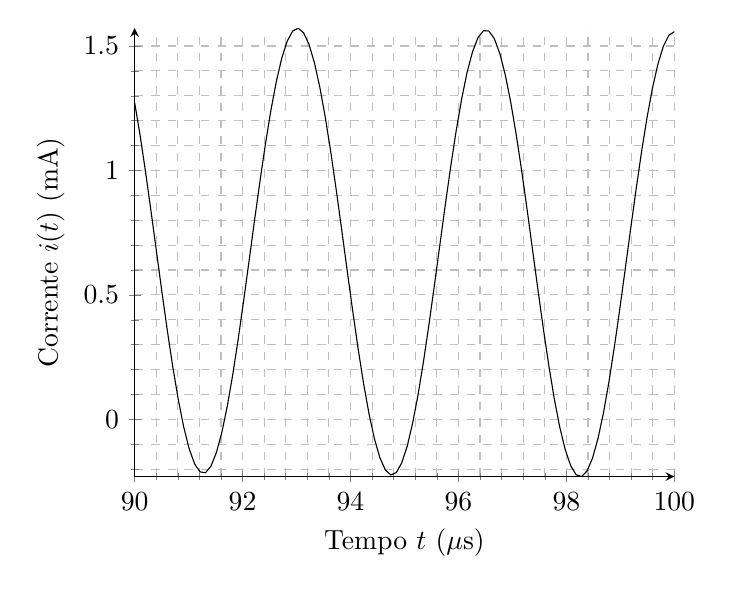
\begin{tikzpicture}
            \begin{axis}[
                axis lines = left,
                xlabel = {Tempo $t$ ($\mu$s)},
                ylabel = {Corrente $i(t)$ (mA)},
                grid style=dashed,
                grid=both,
                minor tick num=4
            ]

            \addplot[
                domain=90:100, 
                samples=100, 
                color=black
            ]
            {0.896*cos(deg(1.8*x-180)) + 0.893*e^(-0.003*x)};
            
            %\addplot [only marks,mark=*,dashed,color=darkgray] coordinates { (\fnum,2*pi*1.8/sqrt(2)};
            %\node[label={160:{\color{darkgray} $(f_{n1},\frac{Q_0}{\sqrt{2}})$}},inner sep=2pt] at (0.956757,7.997189) {};
            
            %\addplot [only marks,mark=*,dashed,color=darkgray] coordinates { (\fndois,2*pi*1.8/sqrt(2)};
            %\node[label={55:{\color{darkgray} $(f_{n2},\frac{Q_0}{\sqrt{2}})$}},inner sep=2pt] at (1.045186,7.997189) {};
            
            %\addplot +[mark=none,color=darkgray,dashed] coordinates {(\fnum, 0.5) (\fnum, 2*pi*1.8)};
            
            %\addplot +[mark=none,color=darkgray,dashed] coordinates {(\fndois, 0.5) (\fndois, 2*pi*1.8)};
            
            %\addlegendentry{}
            \end{axis}
        \end{tikzpicture}
\caption{Proximidade entre os valores aproximados e os valores obtidos através do processo \textit{iterativo}.} \label{fig:proximidade} 
\end{figure}
\fi
%//==============================--D--==============================//%
\clearpage
\subsubsection*{(d) Considere agora que se desliga o gerador quando a tensão vai a passar por zero de valores negativos para positivos, supondo que o circuito está em regime forçado. Determine a solução para $i(t)$, calculando o valor inicial da corrente $I_0$ e a constante de tempo $\tau$.}
\label{subsubsec_d}
\paragraph{Resposta:}
Naturalmente, como consequência imediata da remoção da tensão do gerador, verifica-se que a solução do regime forçado é nula, i.e., $i_f(t) \equiv 0$, $\forall t$.

Com a aplicação da Lei de Indução verifica-se uma equação diferencial \text{homogénea} tal como esperado:
$$
    \overrightarrow{\nabla} \times \overrightarrow{E} = -\dfrac{\partial}{\partial t}\overrightarrow{B} \implies L \dfrac{di(t)}{dt} + i(t)R = 0
$$

A forma da solução desta equação já é conhecida de \hyperref[subsubsec_b]{\underline{2.1} (b)}; é para além disto adiantado que a constante de tempo $\tau$ se mantém inalterada (como seria de esperar), seja $\tau = 0.(3)$ ms.

Para a nova situação, verifica-se a solução geral:
$$
    i(t) = i_n(t) = I_0\cdot e^{-t/\tau}\ \text{A}
$$

Sequencialmente, para determinar $I_0$ é necessário determinar os instantes em que o gerador passa por zero de valores negativos para positivos:
$$
    u_g(t_0) = U_g \cos{(\omega t + \alpha)}\text{, e como $\alpha = -\pi/2$} \implies u_g(t) = U_g \sin{(\omega t)}\ \text{V}
$$

Por conseguinte, $t_0$ é um ponto da forma: $t_0 = 2k\pi/\omega$, $\forall k \in \mathbb{Z}$. 


Até ao instante $t_0$, o circuito funciona em regime forçado, e assim, devido à continuidade de $i(t)$ que nos é assegurada, faz-se uso da equação da corrente forçada, estabelecida na alínea \hyperref[subsubsec_b]{\underline{2.1} (b)}, para calcular a amplitude neste dado instante.

Visto que não ocorrem saltos energéticos infinitos, voltamos ao resultado bastante familiar:
$$
    i(t_0^-) = i(t_0^+) = I_0 \iff I_0 = 0.634 \sqrt{2}\cdot \cos{(\omega t_0 - 3.046)}
$$

$$
    \implies I_0 = 0.634 \sqrt{2}\cdot \cos{(2k\pi-3.046)} \approx -0.893\ \text{mA, }\forall k \in \mathbb{Z}
$$
Em suma, a solução para $i(t)$ é: 
$$
    \therefore i(t) = I_0\cdot e^{-t/\tau} \approx -0.893\cdot e^{-3000t}\ \text{mA}\text{, }\forall t \ge t_0
$$
\hfill \ensuremath{\Box}
%//==============================--E--==============================//%
\subsubsection*{(e) Verifique que para $t = \tau$ se tem: \\ $$i(\tau) = \dfrac{I_0}{e}$$}
\label{subsubsec_e}
\paragraph{Resposta:} Trivialmente verificado por substituição direta na expressão deduzida na alínea anterior:

$$
    i(t) = I_0\cdot e^{-t/\tau} \implies i(\tau) = I_0\cdot e^{-\tau/\tau} = I_0\cdot e^{-1} = \frac{I_0}{e}\ \text{A}
$$
\hfill \ensuremath{\Box}
%//==============================--@--==============================//%
    \clearpage
\def\delequal{\mathrel{\ensurestackMath{\stackon[1pt]{=}{\scriptstyle\Delta}}}}
%//==============================--@--==============================//%
\subsection*{\underline{2.2} Circuito RLC-Série}
%//==============================--A--==============================//%
\subsubsection*{(a) Estabeleça a equação para a corrente ${i}$ em valores instantâneos para ${t \ge 0}$ em função do coeficiente de amortecimento ${\beta}$ e da frequência angular das oscilações não amortecidas ${\omega_0}$.
Calcule $\omega_0$.}
\label{subsubsec_a2}
\paragraph{Resposta:}
Escolhendo o caminho fechado conforme o enunciado (interruptor comutado), com o sentido coincidente com o da corrente convencionado, obtém-se, através da Lei de Indução:
$$
    \overrightarrow{\nabla} \times \overrightarrow{E} = -\dfrac{\partial}{\partial t}\overrightarrow{B} \implies i(t)\cdot (R' + R_G) + \frac{1}{C} \int i(t)\, dt + L \frac{di(t)}{dt} = 0
$$

Para obter a ilustre EDO linear de 2\textsuperscript{\underline{a}} ordem homogénea, é simplesmente necessário derivar em ordem a $t$, i.e.:
$$
    i(t)\cdot (R' + R_G) + \frac{1}{C} \int i(t)\, dt + L \frac{di(t)}{dt} = 0 \implies  L \frac{d^2i(t)}{dt^2} + \frac{di(t)}{dt}\cdot R + \frac{1}{C}\cdot i(t) = 0
$$

$$
    \iff \frac{d^2i(t)}{dt^2} + \frac{R}{L} \cdot \frac{di(t)}{dt} + \frac{1}{CL}\cdot i(t) = 0
$$

Por comparação direta com a forma canónica $\dfrac{d^2i(t)}{dt^2} + 2\beta \cdot \dfrac{di(t)}{dt} + \omega_{0}^{2}\cdot i(t) = 0$, pode-se concluir celeremente:

$$
    \begin{cases}
        \beta = \dfrac{R}{2L} \\
        \omega_0 = \dfrac{1}{\sqrt{LC}} = \dfrac{\sqrt{LC}}{LC} = 50\ \text{krad s}^{-1}
    \end{cases}
$$
\hfill \ensuremath{\Box}
%\footnotetext[2]{Do enunciado temos que $R = R' + R_G$.}
%//==============================--B--==============================//%
\subsubsection*{(b) Estabeleça as condições iniciais para o regime que se obtém para ${t \ge 0}$. Caracterize o regime forçado para ${t \ge 0}$.}
\label{subsubsec_b2}
\paragraph{Resposta:}
Caracteristicamente de sistemas reais, é de esperar que não ocorram saltos energéticos infinitos derivados de descontinuidades de $u_C(t)$ e $i_L(t)$.
$$
    p_C = \frac{d}{dt}W_e(t) \to \infty;\ \ \ p_L = \frac{d}{dt}W_m(t) \to \infty
$$

Esta situação é, naturalmente, fisicamente absurda, e não se pode evitar a conclusão óbvia de que $u_C(t)$ e $i_L(t)$ se verificam inalterados no instante de comutação do interruptor. Isto é:
$$
    u_C(0^+) = u_C(0^-);\ \ \ i_L(0^+) = i_L(0^-) 
$$

Através da Lei de Indução, salientando que se trata de um regime estacionário para $t < 0$, e que se trata de um circuito em série, concluem-se deste modo as condições iniciais:
$$
    \begin{cases}
        \bar{U}_G = \bar{U}_C + \bar{U}_L \\
        i(t) = i_L(t)
    \end{cases}
    \implies
    \begin{cases}
        u_C(0) = U_G(0) = 4\ \text{V} \\
        i(0^+) = i(0^-) = i(0) = 0\ \text{A}
    \end{cases}
$$

Assim, ao comutar o interruptor, para $t > 0$, estamos perante um regime livre da influência do gerador. 

Como esta influência foi removida, a solução dos problemas de valor inicial deve tender para zero há medida que o tempo se alastra (existem elementos dissipativos no circuito). Pelo que, naturalmente se verifica:
$$
    \begin{cases}
        %i_f(t) = \lim\limits_{t \to \infty} i(t) = 0\ \text{A}\\
        %u_f(t) = \lim\limits_{t \to \infty} u_C(t) = 0\ \text{V}
        i_f(t) = 0\ \text{A}\\
        u_f(t) = 0\ \text{V}
    \end{cases}
$$
\hfill \ensuremath{\Box}
%//==============================--C--==============================//%
\subsubsection*{(c) Discuta os tipos de solução que pode obter para o regime livre com ${R}$ variável.}
\label{subsubsec_c2}
\paragraph{Resposta:} 
Desprovido da influência do gerador, o circuito apresenta somente um regime livre que já foi introduzido, i.e.:
$$
    \dfrac{d^2i(t)}{dt^2} + 2\beta \cdot \dfrac{di(t)}{dt} + \omega_{0}^{2}\cdot i(t) = 0
$$

Esta EDO linear de 2\textsuperscript{\underline{a}} ordem homogénea é de resolução imediata recorrendo ao seu polinómio caracteristico:
$$
    s^2 + 2\beta s + \omega_0^2 = 0 \implies s = -\beta \pm \sqrt{\beta^2 - \omega_0^2}
$$

Aproveitando as relações\footnotemark[2] deduzidas na alínea \hyperref[subsubsec_a2]{\underline{2.2} (a)}, imediatamente se conclúi, ao analizar o binómio discriminante, que estamos perante três possíveis cenários:

\begin{itemize}
  \item $\beta > \omega_0 \iff R > 2\sqrt{\dfrac{L}{C}}$: estamos perante um regime aperiódico fortemente amortecido e, como tal, as raízes são reais e diferentes (a solução para $i$ seriam duas exponenciais decadentes).   
  \item $\beta = \omega_0 \iff R = 2\sqrt{\dfrac{L}{C}}$: estamos perante um regime aperiódico \textit{criticamente} amortecido (limite), neste caso temos uma raiz dupla real (a solução toma a forma de duas exponenciais decadentes em que uma é multiplicada por $t$).
  \item $\beta < \omega_0 \iff R < 2\sqrt{\dfrac{L}{C}}$: estamos perante um regime oscilatório amortecido, visto que são encontradas duas raizes complexas conjugadas (a solução é da forma de uma sinusoide multiplicada por uma exponencial decadente).
\end{itemize}
\hfill \ensuremath{\Box}

\footnotetext[2]{Especificamente $\beta = R/2L$, dado que estamos a realizar um \textit{gedankenexperiment} em que $R$ é uma variável.}
%//==============================--D--==============================//%
\subsubsection*{(d) Para ${R = 100\ \Omega}$, calcule o coeficiente de amortecimento ${\beta}$ e verifique que a solução é do tipo oscilatório amortecido. Calcule ${\omega = 2\pi/T}$ sendo ${T}$ o período de isocronismo. Verifique que: \\ $$ A_1/A_2 = A_2/A_3 = \cdots = (A_1/A_n)^{\frac{1}{n-1}} = e^{\lambda}$$ Determine $\lambda$. Determine $i(t)$ e $u_C(t)$ tendo em conta as condições iniciais estabelecidas em b).}
\label{subsubsec_d2}
\paragraph{Resposta:}
Utilizando diretamente as expressões obtidas anteriormente:
$$
    \beta = \frac{R}{2L} = \frac{5}{2\cdot 10\cdot 10^{-3}} = 5\ \text{kNp}\ s^{-1}
$$
\hfill \ensuremath{\Box}

Desta forma, encontramo-nos de facto num regime oscilatório amortecido. Tal afirmação verifica-se imediatamente com o discutido na alínea precedente juntamente o resultado obtido para a frequência natural na alínea \hyperref[subsubsec_a2]{\underline{2.2} (a)}, i.e.:
$$
    \beta < \omega_0 \iff 5\cdot 10^3 < 50\cdot 10^3 \implies [(5 < 50) \land 1] = 1 
$$
\hfill \ensuremath{\Box}

Posto isto, e tendo em conta que o regime transitório é puramente livre, temos que $i(t)$ é da forma:
\begin{equation}
    \label{eq2}
    i(t) = \mathbb{R}e\{\bar{I} e^{st} \} = Ie^{-\beta t}\cos{(\omega t + \theta)}
\end{equation}

$$
    \begin{cases}
        \omega = \sqrt{\omega_0^2 - \beta^2} \approx 49.749\ \text{krad s}^{-1} \\
        s = -\beta + j\omega = \omega_0\ e^{j\delta};\ \ \ \delta = \pi - \arctan{\left(\frac{\omega}{\beta}\right)} = 1.573\ \text{rad}
    \end{cases}
$$

Em que $\omega$ é a frequência angular das oscilações amortecidas e $\bar{I} = Ie^{j\theta}$. Assim, o período de isocronismo é facilmente deduzido:
$$
    \omega = \frac{2\pi}{T} \implies T = \frac{2\pi}{\omega} \approx 126.298\ \mu\text{s}
$$
\hfill \ensuremath{\Box}

De modo a verificar a igualdade enunciada: $A_1/A_2 = \cdots = (A_1/A_n)^{1/(n-1)} = e^{\lambda}$, com $\lambda = \beta T/2$; considera-se o facto de que de $T/2$ em $T/2$, a função regida pela sinusoide encontra ora dois zeros consecutivos, ou dois extremos consecutivos. 

Assim, denominando por $t_n$ o instante em que se verifica um extremo, temos:
$$
    t_{n+1} = t_n + \frac{T}{2} \implies
    \begin{cases}
        i(t_n) = Ie^{-\beta t_n}\cos{(\omega t_n + \theta)}\\
        i(t_{n+1}) = Ie^{-\beta t_n}e^{-\beta \frac{T}{2}}\cos{(\omega t_n + \pi + \theta)}
    \end{cases}
$$

\clearpage
Sendo então o racio entre duas amplitudes consecutivas:
$$
    \left\vert \frac{i(t_{n})}{i(t_{n+1})} \right\vert = \frac{A_{n}}{A_{n+1}} = \left\vert \frac{Ie^{-\beta t_n}\cos{(\omega t_n + \theta)}}{-Ie^{-\beta t_n}e^{-\beta \frac{T}{2}}\cos{(\omega t_n + \theta)}} \right\vert
$$

$$
    \therefore \frac{A_{n+1}}{A_{n}} = e^{\beta \frac{T}{2}} = e^{\lambda}
$$

Note-se que $t_{n+1} = t_n + T/2$ é uma progressão aritmética de razão $T/2$. Assim, temos:
$$
    t_{n} = t_1 + (n-1)\cdot \frac{T}{2} \implies t_1 = t_{n} + (1-n)\frac{T}{2}
$$

Então:
$$
    \left\vert \frac{i(t_{1})}{i(t_{n})} \right\vert = \frac{A_{1}}{A_{n}} = \left\vert \frac{Ie^{-\beta t_{n}}e^{(n-1)\beta\frac{T}{2}}\cos{(\omega t_{n} - n\pi + \pi + \theta)}}{-Ie^{-\beta t_{n}}\cos{(\omega t_{n+1} + \theta)}} \right\vert
$$

$$
    \therefore \frac{A_{1}}{A_{n}} = e^{(n-1)\beta\frac{T}{2}} \implies \left(\frac{A_{1}}{A_{n}}\right)^{1/(n-1)} = e^{\beta\frac{T}{2}} = e^{\lambda} 
$$

Finalmente, conclúi-se:
$$
    \therefore \frac{A_n}{A_{n+1}} = \left(\frac{A_1}{A_n}\right)^{1/(n-1)} = e^{\lambda};\ \ \ \lambda = \beta\frac{T}{2} \approx 315.745\ \text{mNp}
$$
\hfill \ensuremath{\Box}

Relembrando a \hyperref[eq2]{equação (3)} e as condições iniciais obtidas na alínea \hyperref[subsubsec_b2]{\underline{2.2} (b)}, encontra-se sem grande resistência o argumento $\theta$ da corrente:
$$
    i(t) = Ie^{-\beta t}\cos{(\omega t + \theta)} \implies i(0) = I\cos{(\theta)} = 0 \implies \theta = \frac{\pi}{2} + k\pi\text{, }\forall k \in \mathbb{Z} 
$$

Encontramo-nos perante um circuito em série, logo:
$$
    u_C(t) = \frac{1}{C}\int i(t)\, dt = \frac{1}{C}\int \mathbb{R}e\{\bar{I} e^{st} \}\, dt = \frac{1}{C}\mathbb{R}e\{\frac{1}{s}\bar{I} e^{st}\}
$$

$$
    \implies u_C(t) = \frac{I}{\omega_0 C}e^{-\beta t}\cos{(\omega t + \theta - \delta)}
$$

Verifica-se que no instante de comutação do interruptor $u_C(0) = 4\ \text{V}$, e assim facilmente se obtem o valor da amplitude I. Seja $k = 0$, então:
$$
    u_C(0) = \frac{I}{\omega_0 C}\cos{(\theta - \delta)} \implies I = \frac{4 \cdot \omega_0 C}{\cos{(\theta - \delta)}} \approx  8.0\ \text{mA}
$$

Em suma, temos as seguintes soluções:
$$
    i(t) = Ie^{-\beta t}\cos{(\omega t + \theta)};\ \ \ u_C(t) = \frac{I}{\omega_0 C}e^{-\beta t}\cos{(\omega t + \theta - \delta)}
$$
\hfill \ensuremath{\Box}

%//==============================--E--==============================//%
\clearpage
\subsubsection*{(e) Calcule $R_0 = R$ de modo que a solução do regime livre seja do tipo aperiódico limite. Determine $i(t)$. Determine igualmente o valor mínimo de $i\ (i_{min})$ e o instante em que ocorre $(t_{min})$.}
\label{subsubsec_e2}
\paragraph{Resposta:}
Com os resultados da alínea \hyperref[subsubsec_c2]{\underline{2.2} (c)} é de imediato calcular a resistência $R_0$ que nos leva a uma solução do polinómio característico da equação diferencial com raiz dupla (isto é, um regime aperiódico limite; dado que $\beta = \omega_0$):
$$
    R_0 = 2\sqrt{\frac{L}{C}} = 1000\ \Omega \implies \beta = 50\ \text{kNp s}^{-1}
$$

Assim, naturalmente, a solução encontrada para $i(t)$ é nos moldes:
\begin{equation}
    i(t) = (I' + t I'')e^{-\beta t}    
\end{equation}

Em seguinda, calculam-se as amplitudes $I'$ e $I''$, com uso das condições iniciais discutidas anteriormente:
$$
    i(0) = 0 \implies I' = 0\ \text{A} \implies i(t) = t I'' e^{-\beta t} 
$$

Do mesmo modo, sabe-se que $u_C(0) = 4\ \text{V}$, e por aplicação direta da Lei de Indução, temos:
$$
    u_C(0) = 4 \implies -R_0 i(0) - L \frac{di(0)}{dt} = 4 \iff \frac{di(0)}{dt} = -400\ \text{A}
$$

$$
    \frac{di(t)}{dt} = -I''(\beta t - 1)e^{-\beta t} \implies \frac{di(0)}{dt} = -400 \iff I'' = -400\ \text{A}
$$

De justa forma, obtem-se a expressão final para $i(t)$ no regime aperiódico limite:
$$
    \therefore i(t) = -400t e^{-\beta t}\text{, com }\beta = 50\ \text{kNp s}^{-1}
$$
\hfill \ensuremath{\Box}

Logicamente, visto que $i(t)$ é uma função \textit{estritamente} decrescente até ao seu valor mínimo e que após passar este ponto tende para zero (não obstante dado o regime livre), obtemos trivialmente o seu valor mínimo através do zero da sua 1\textsuperscript{\underline{a}} derivada.

Como nos lembra a Análise real:
$$
    \frac{di(t)}{dt} = -I''(\beta t - 1)e^{-\beta t} = 0 \iff t = \frac{1}{\beta} = \frac{2L}{R_0} = 20\ \mu\text{s}
$$

Então, por fim:
$$
    \begin{cases}
        t_{\text{min}} = 20\ \mu\text{s}\\
        i_{\text{min}} = i(t_{\text{min}}) = \dfrac{-1}{125e} \approx -2.943\ \text{mA}
    \end{cases}
$$
\hfill \ensuremath{\Box}
%//==============================--@--==============================//%
    %% attachments
    \newpage
    %\input{sections/anexo}

\end{document}
